\chapter{Results}\label{cha:results}
Here the results of the thesis will be presented.
This includes figures of the voxelization, graphs of the performance and data of the error analysis.

\section{Voxelization}
The result of the floating-point voxelization can be seen in \figref{fig:voxelization}.
The same voxelization of the integer versions is shown in \figref{fig:voxelization-ilv} and \figref{fig:voxelization-bresenham}.
The figures show voxelizations between 16-512 resolution, but resolutions up to 2048 were possible.
However, due to the aliasing in the rendering, showing the result of such high resolution would be meaningless.

All the models in the voxelization were scaled to fit the voxel grid perfectly, without changing the aspect ratio of them.
More figures of the voxelizations can be found in \appref{app:voxelizations}.

\section{Performance Analysis}
The performance of each of the models can be seen in \figref{fig:performance-model}.
The same data is plotted for each of the algorithms in \figref{fig:performance-alg}.
Each data point is the average time to voxelize the models in a total of 100 iterations.
The raw performance data can be found in \appref{app:performance-data}.

One unsolved problem about the performance data is that the timings improved after iterating the voxelization multiple times.
As an example, \figref{fig:performance-runs} shows how the timings varied after a certain amount of iterations.
The time for a single voxelization decreased by around 50\%.
This will further be discussed in the next chapter.
Since the data seem to converge to a certain time, the average of the last 100 out of the 1000 iterations were used as the final measurement in the previously mentioned graphs.
% \begin{table}[ht]
%   \centering
% \begin{tabular}{l|l|lllll}
%   Model & Algorithm & 128 & 256 & 512 & 1024 & 2048 \\
%   \hline
% \multirow{2}{*}{Monkey} & ILV       & 20\% & 60\% & 56\% & 43\% & 32\% \\
%  & Bresenham & 40\% & 76\% & 59\% & 37\% & 20\% \\
% \hline
% \multirow{2}{*}{Bunny} & ILV       & 210\% & 231\% & 86\% & 35\% & 25\% \\
%  & Bresenham & 410\% & 420\% & 156\% & 69\% & 48\% \\
% \hline
% \multirow{2}{*}{Dragon} & ILV       & 215\% & 255\% & 250\% & 235\% & 133\% \\
%  & Bresenham & 448\% & 518\% & 495\% & 443\% & 234\% \\
% \end{tabular}
% \caption{Runtime increase for the integer versions relative to RLV. All values are rounded to the nearest whole number.}\label{tab:performance-data}
% \end{table}

% \FloatBarrier

\input{fig/voxelization.fig}

\voxelizationfig{bunny}{rlv}{Floating-point voxelization using RLV of the Stanford bunny at 16, 32, 64, 128, 256 and 512 resolution}{fig:voxelization}
\voxelizationfig{bunny}{ilv}{Integer voxelization using ILV of the Stanford bunny at 16, 32, 64, 128, 256 and 512 resolution}{fig:voxelization-ilv}
\voxelizationfig{bunny}{bre}{Integer voxelization using Bresenham of the Stanford bunny at 16, 32, 64, 128, 256 and 512 resolution}{fig:voxelization-bresenham}
\input{fig/performance-model.fig}
\input{fig/performance-alg.fig}

\input{fig/performance-runs.fig}

\FloatBarrier

\section{Error Analysis}
An example of the difference between RLV and ILV can be seen in \figref{fig:compare}. 
It shows a comparison where voxels are colored depending on if they exist in both voxelizations or only one of them.
More comparisons can be seen in \appref{app:compare-error}, where all models and resolutions between 16-512 are shown. 

The Jaccard distance between the different versions of the voxelizations can be seen in \tabref{tab:error-data}. 

\begin{figure}[h]
\centering
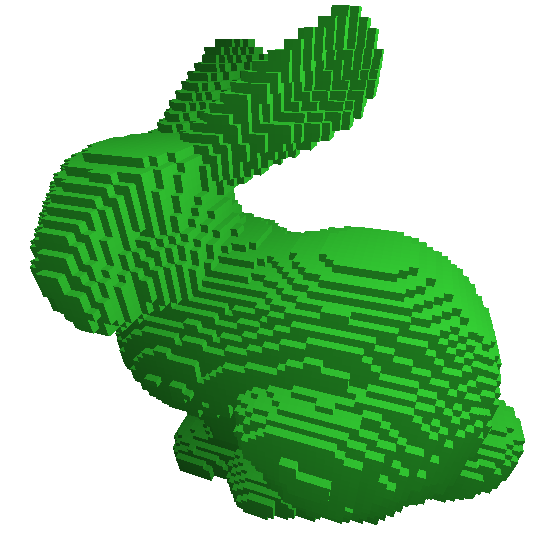
\includegraphics[width=0.3\textwidth]{fig/voxelization/bunny/bunny_rlv_64.png}
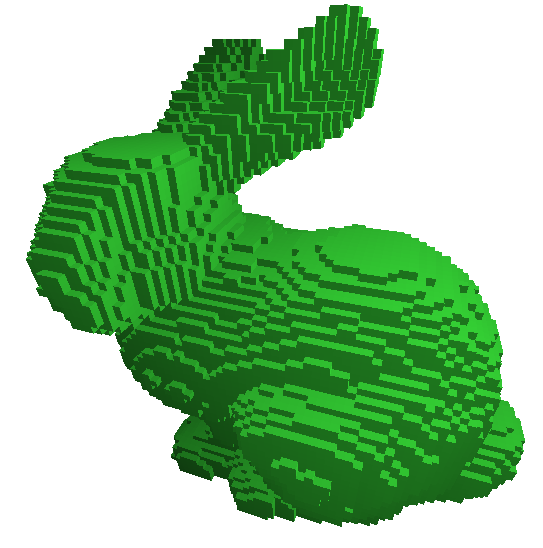
\includegraphics[width=0.3\textwidth]{fig/voxelization/bunny/bunny_ilv_64}
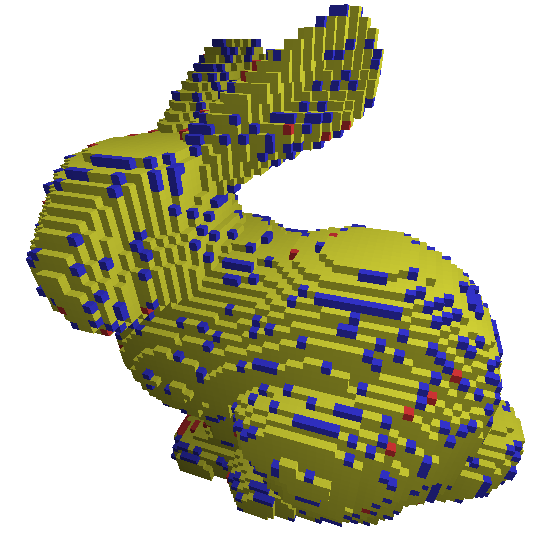
\includegraphics[width=0.3\textwidth]{fig/voxelization/bunny/bunny_rlv_ilv_64}
\caption{
  Difference between floating-point and integer voxelization.
  The left-most figure uses RLV, the middle uses ILV and the right-most is the union between them.
  The yellow voxels are in both versions.
  The red voxels are only in the RLV version.
  The blue voxels are only in the ILV version.
}\label{fig:compare}
\end{figure}

\begin{table}[h]
  \centering
\begin{tabular}{l|l|lllll}
  Model & Algorithm & 128 & 256 & 512 & 1024 & 2048 \\
  \hline
         & RLV/ILV & 21.63\% & 22.10\% & 22.51\% & 22.98\% & 23.53\% \\
  Monkey & RLV/Bre & 21.89\% & 22.30\% & 23.04\% & 23.67\% & 24.16\% \\
         & ILV/Bre & 4.72\% & 5.62\% & 5.58\% & 5.35\% & 5.21\% \\
  \hline
         & RLV/ILV & 19.65\% & 20.62\% & 22.12\% & 22.59\% & 22.8\% \\
  Bunny  & RLV/Bre & 19.66\% & 21.21\% & 22.30\% & 22.94\% & 23.21\% \\
         & ILV/Bre & 0.07\% & 4.57\% & 4.77\% & 5.59\% & 5.23\% \\
  \hline
         & RLV/ILV & 9.42\% & 15.65\% & 21.28\% & 21.87\% & 22.75\% \\
  Dragon & RLV/Bre & 9.42\% & 15.67\% & 21.40\% & 22.52\% & 23.29\% \\
         & ILV/Bre & 0.00\% & 0.05\% & 1.09\% & 3.84\% & 5.22\% \\
\end{tabular}
\caption{The Jaccard distance between the different algorithms, with varying models and resolution. Bre in the table is short for Bresenham. All errors are rounded to the nearest hundredth.}\label{tab:error-data}
\end{table}

